
\documentclass[UTF8,11pt]{ctexart}
\usepackage[a4paper,margin=2.3cm]{geometry}
\usepackage{amsmath,amssymb,mathtools}
\usepackage{physics}
\usepackage{graphicx}
\usepackage{booktabs}
\usepackage{enumitem}
\usepackage{xcolor}
\usepackage{listings}
\usepackage[hidelinks]{hyperref}
\usepackage{caption}
\captionsetup{font=small}
\lstset{
  basicstyle=\ttfamily\small,
  breaklines=true,
  frame=single,
  columns=fullflexible,
  keepspaces=true,
  showstringspaces=false
}
\setlength{\parskip}{0.45em}
\setlength{\parindent}{2em}
\numberwithin{equation}{section}

\title{\(^{171}\mathrm{Yb}\) UV Rydberg CZ 片段的热涨落响应}
\author{}
\date{\today}

\begin{document}
\maketitle

\begin{abstract}
本文整理固定 \(^{171}\mathrm{Yb}\) UV Rydberg controlled-Z (CZ) 控制片段在有限温度下的热噪声响应。该片段是 shelved control--Rydberg excitation stage，不是完整实验门序列；本文只隔离热运动进入有效 Hamiltonian 的主要通道：相对位置涨落诱导的 blockade shift 分布，以及沿 UV 波矢方向速度涨落诱导的 common-mode Doppler detuning。固定 pulse 是在只考虑 Rydberg decay 的 no-jump 模型中按 time-optimal 思路得到的 Gaussian-edge phase-only pulse，没有针对热噪声重新优化。在 \(\bar n=0.25\) 对应的 \(T_\mathrm{ref}\simeq1.49\,\mu\mathrm{K}\) 附近，thermal excess infidelity 约为 \(3.21\times10^{-5}\)，低于 fixed-pulse baseline \(7.19\times10^{-4}\)。升温至 \(30\,\mu\mathrm{K}\) 时，thermal excess 增至 \(7.04\times10^{-4}\)，与 baseline 同量级。
\end{abstract}

\noindent\textbf{关键词：} \(^{171}\mathrm{Yb}\)；Rydberg CZ gate；thermal motion；blockade shift；Doppler detuning；process fidelity

\section{问题设定}

固定 UV CZ 片段面对的 thermal response 可以写成一条链：
\[
\text{thermal motion}
\longrightarrow
\{q,\delta_1,\delta_2\}
\longrightarrow
H(t;q,\delta_1,\delta_2)
\longrightarrow
U_\mathrm{no\ jump}
\longrightarrow
F_\mathrm{pro}.
\]
这里 \(q\) 是两原子沿连线方向的相对位移，\(\delta_i\) 是第 \(i\) 个原子的 Doppler detuning。相对位移改变 Rydberg pair interaction \(B(R)\)，速度涨落改变 UV excitation 的有效失谐。本文在正文中只保留与 fidelity response 直接相关的物理图像；温度换算、尺度推导、fidelity 定义和采样细节放在附录 \hyperref[app:nbar-temperature]{A}--\hyperref[app:numerics]{D}。

\section{有效模型与固定 pulse}
\subsection{Reduced basis}

每个原子的相关态粗略记为
\[
|0\rangle,\qquad |c\rangle,\qquad |r\rangle,
\]
其中 \(|0\rangle\) 是该 UV 片段中不参与 Rydberg excitation 的 branch，\(|c\rangle\) 是会被 UV 光耦合到 Rydberg 态的 shelved control branch，\(|r\rangle\) 是目标 Rydberg state。数值模型采用交换对称 reduced basis：
\begin{lstlisting}
|00>, |0c>, |0r>, |cc>, |W_cr>, |rr>
\end{lstlisting}
其中
\[
|W_{cr}\rangle=\frac{|cr\rangle+|rc\rangle}{\sqrt{2}}.
\]
理想 CZ 条件是 pulse 结束后 diagonal branches 回到自身，只积累相位，并满足
\[
\theta_{cc}-2\theta_{0c}+\theta_{00}=\pi\quad (\mathrm{mod}\ 2\pi).
\]

\subsection{Pulse 形状：time-optimal phase-only control}

UV laser 的复 Rabi frequency 写成
\[
\Omega(t)=\Omega_\mathrm{max}A(t)e^{i\phi(t)}.
\]
当前使用的 pulse 参数为
\[
\Omega_\mathrm{max}/2\pi=10\,\mathrm{MHz},\qquad
T_\mathrm{gate}=170\,\mathrm{ns},\qquad
N_t=64.
\]
其中 \(A(t)\) 是固定 Gaussian-edge envelope，edge time 为 \(40\,\mathrm{ns}\)；\(\phi(t)\) 是 64-slot phase sequence。这个 pulse 来自只考虑 Rydberg decay 的 no-jump 模型下的 time-optimal phase-only 优化：优化目标是固定最大 Rabi 频率和 Gaussian edge 后，寻找最短且达到 fidelity threshold 的相位波形。它没有把 thermal blockade fluctuation 或 Doppler detuning 放入优化目标，因此本文是在固定该 pulse 后做 thermal response analysis。

\begin{figure}[htbp]
\centering

\includegraphics[width=0.78\linewidth]{figures/gaussian_edge_envelope_nominal.png}
\caption{固定 UV pulse 的 Gaussian-edge amplitude envelope。}
\end{figure}

\begin{figure}[htbp]
\centering

\includegraphics[width=0.78\linewidth]{figures/nominal_timeoptimal_phase_trace.png}
\caption{固定 UV pulse 的 unwrapped phase sequence。该相位序列是在只考虑 decay 的 time-optimal scan 中选出的 nominal row。}
\end{figure}

\subsection{Hamiltonian 与 no-jump decay}

在 rotating frame 中，控制项可以写成
\[
H_\mathrm{ctrl}(t)=
\frac{\Omega_\mathrm{max}A(t)}{2}
\left[e^{i\phi(t)}|0r\rangle\langle0c|+\mathrm{h.c.}\right]
+
\frac{\Omega_\mathrm{max}A(t)}{\sqrt{2}}
\left[e^{i\phi(t)}|W_{cr}\rangle\langle cc|
+e^{i\phi(t)}|rr\rangle\langle W_{cr}|+\mathrm{h.c.}\right].
\]
有限 blockade 和 common-mode Rydberg detuning 分别进入 diagonal drift：
\[
H_B=B(R)|rr\rangle\langle rr|,
\]
\[
H_\delta=\delta |0r\rangle\langle0r|+\delta |W_{cr}\rangle\langle W_{cr}|+2\delta |rr\rangle\langle rr|.
\]
Rydberg decay 通过 no-jump 非厄米项加入：
\[
G_\mathrm{decay}
=-\frac12\mathrm{diag}(0,0,\gamma,0,\gamma,2\gamma)/\Omega_\mathrm{max}.
\]
因此传播器是 conditioned-on-no-jump propagator，而非完整 Lindblad master equation。

\subsection{Fidelity 读数}

对固定 UV phase sequence 和给定 \(B,\delta\)，取三个 diagonal branches 的 no-jump amplitude
\[
z=\{z_{00},z_{0c},z_{cc}\}.
\]
静态 blockade scan 中允许重新拟合 virtual-\(Z\) phases \(\alpha,\beta\)，计算 phase-corrected restricted CZ process fidelity：
\[
F_\mathrm{pro}
=\frac{1}{16}\left|
z_{00}e^{-i\alpha}
+2z_{0c}e^{-i(\alpha+\beta)}
-z_{cc}e^{-i(\alpha+2\beta)}
\right|^2.
\]
温度扫描中 thermal shifts 是 shot-to-shot random，因此使用固定 nominal virtual-\(Z\) phases，并报告 baseline-subtracted excess infidelity。标称点的 baseline 为
\[
I_0=1-F_0=7.1897674\times10^{-4}.
\]
完整的 process fidelity、active population、no-jump average fidelity 和 fixed virtual-\(Z\) averaging 定义见附录~\ref{app:fidelity-definition}。

\section{热运动噪声模型与 fidelity 响应}
\subsection{位置涨落 \(\rightarrow\) blockade 分布 \(\rightarrow\) fidelity 响应}

两原子标称间距为 \(R_0=3\,\mu\mathrm{m}\)。若相对热位移为 \(q\)，则
\[
R=R_0+q,
\qquad
B(R)=B_0\left(\frac{R_0}{R}\right)^6
=\frac{B_0}{(1+q/R_0)^6}.
\]
线性化给出 \(\Delta B/B_0\simeq -6q/R_0\)，完整推导见 \hyperref[app:blockade-scale]{附录 B}。参考温度 \(T_\mathrm{ref}=1.490969\,\mu\mathrm{K}\) 下，\(q\) 的一维 Gaussian 分布通过上式映射成下图的 blockade distribution。

\begin{figure}[htbp]
\centering
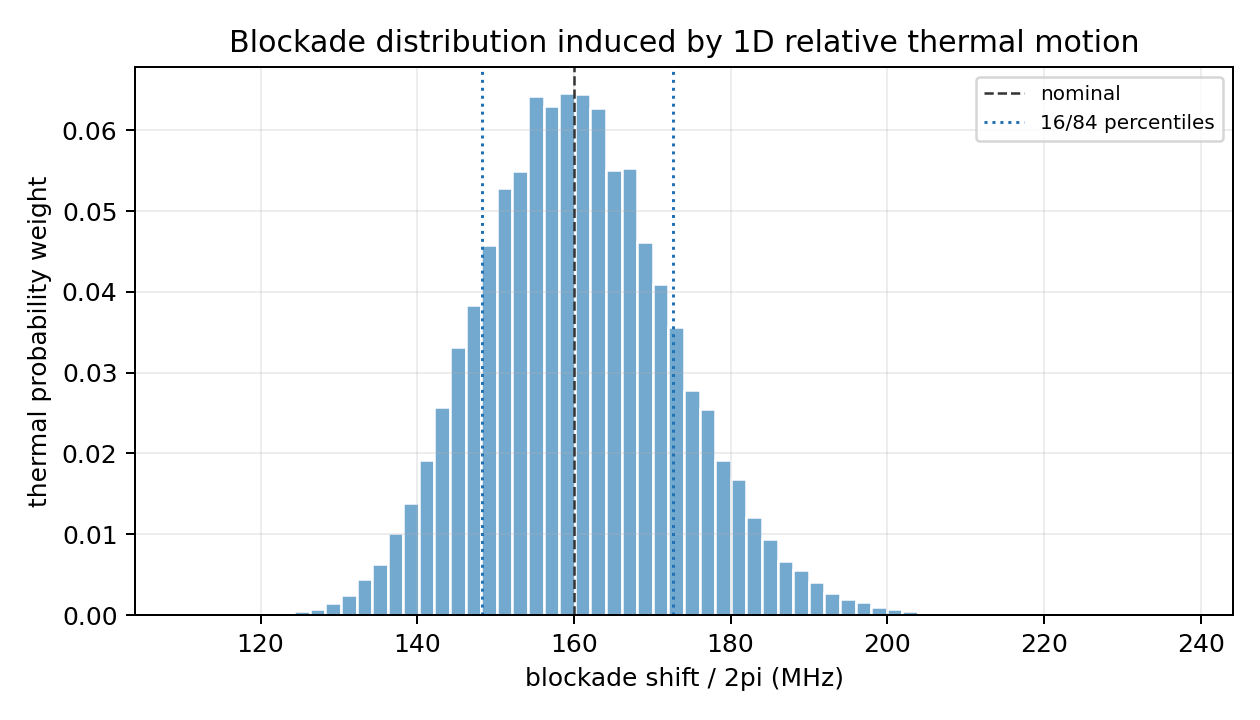
\includegraphics[width=0.86\linewidth]{figures/thermal_blockade_distribution_estimate.png}
\caption{Blockade distribution induced by 1D relative thermal motion. 黑色虚线为标称 \(B_0/h=160\,\mathrm{MHz}\)，蓝色虚线为 \(16/84\) 分位点。}
\end{figure}

参考温度下该分布的 mean 为 \(160.550\,\mathrm{MHz}\)，standard deviation 为 \(12.346\,\mathrm{MHz}\)，\(16/84\) 分位点为 \(148.257/172.675\,\mathrm{MHz}\)。在这个分布上平均 phase-corrected process fidelity 得到
\[
F_\mathrm{pro}^{(B\ \mathrm{avg})}=0.999274365878,
\]
即 process infidelity 从标称 \(7.1898\times10^{-4}\) 变为 \(7.2563\times10^{-4}\)。

为了把该分布转换成 fidelity 影响，还需要固定 pulse 的 response function：
\[
B\longmapsto 1-F_\mathrm{pro}(B).
\]
下图展示了这个响应。蓝色阴影是参考温度下的 thermal one-sigma blockade 区间。

\begin{figure}[htbp]
\centering

\includegraphics[width=0.86\linewidth]{figures/thermal_blockade_process_fidelity_response.png}
\caption{Fixed-phase thermal blockade response. 该图只显示 phase-corrected process infidelity 对 blockade shift 的响应。}
\end{figure}

这张图说明 \(B/h=160\,\mathrm{MHz}\) 附近曲线较平，因此参考温度下的 blockade fluctuation 只带来 \(10^{-5}\) 量级额外 infidelity；但如果 blockade 明显降低到 \(120\,\mathrm{MHz}\) 附近，infidelity 会快速上升。

\subsection{Doppler 噪声 \(\rightarrow\) common-mode detuning \(\rightarrow\) fidelity 响应}

一维 thermal velocity distribution 给出
\[
\sigma_v^2(T)=\frac{k_B T}{m}.
\]
对单光子 UV excitation，\(k_\mathrm{UV}=2\pi/\lambda\)，\(\lambda=301.9\,\mathrm{nm}\)，所以单原子 Doppler RMS 为
\[
\frac{\sigma_\delta(T)}{2\pi}=\frac{\sigma_v(T)}{\lambda}
=23.097\sqrt{T_{\mu\mathrm{K}}}\,\mathrm{kHz}.
\]
参考温度下
\[
\frac{\sigma_\delta}{2\pi}=28.20\,\mathrm{kHz},
\qquad
\frac{\sigma_\delta}{\Omega}=2.82\times10^{-3}.
\]
对两个原子定义
\[
\delta_c=\frac{\delta_1+\delta_2}{2},
\qquad
\delta_d=\frac{\delta_1-\delta_2}{2}.
\]
在 symmetric/antisymmetric basis 中，Doppler Hamiltonian 含有
\[
H_D=-\delta_c(|W\rangle\langle W|+|A\rangle\langle A|)
-\delta_d(|W\rangle\langle A|+|A\rangle\langle W|).
\]
当前六态模型只包含 \(|W\rangle\)，没有 \(|A\rangle\)，因此数值结果只纳入 common-mode \(\delta_c\)。这给出参考温度下的 common-mode Doppler excess infidelity
\[
\Delta I_D(T_\mathrm{ref})=1.38\times10^{-5}.
\]
这个数值与 blockade contribution \(\Delta I_B(T_\mathrm{ref})=1.83\times10^{-5}\) 同量级但略小。需要注意，这并不表示完整 Doppler error 一定更小，因为差分 detuning 对 antisymmetric sector 的耦合尚未进入模型。

\subsection{整体 thermal temperature scan components}

把 blockade 与 common-mode Doppler 分开平均后，定义 baseline-subtracted contributions：
\[
\Delta I_B(T)=\langle 1-F_B(q)\rangle_q-I_0,
\qquad
\Delta I_D(T)=\langle 1-F_D(\delta_c)\rangle_{\delta_c}-I_0.
\]
总 thermal excess 与估计总 infidelity 为
\[
\Delta I_\mathrm{thermal}(T)=\Delta I_B(T)+\Delta I_D(T),
\qquad
I_\mathrm{total}(T)=I_0+\Delta I_\mathrm{thermal}(T).
\]
更完整的 fidelity 定义见附录~\ref{app:fidelity-definition}；采样和插值细节见附录~\ref{app:numerics}。

\begin{figure}[htbp]
\centering

\includegraphics[width=0.94\linewidth]{figures/thermal_temperature_scan_infidelity_components.png}
\caption{Thermal temperature scan components. 横轴和纵轴均采用 logarithmic scale。蓝色、橙色、绿色分别为 blockade excess、common-mode Doppler excess 和二者相加；黑色为 baseline 加 thermal excess。淡蓝色背景标出 \(\bar n=0.25\pm0.10\) 对应的温度区间，灰色竖线为 \(\bar n=0.25\) 的参考温度。}
\end{figure}

图中可见，在 \(T_\mathrm{ref}\simeq1.49\,\mu\mathrm{K}\) 附近，thermal excess sum 为 \(3.21\times10^{-5}\)，显著低于 fixed-pulse baseline \(I_0\simeq7.19\times10^{-4}\)。升温到 \(30\,\mu\mathrm{K}\) 时，thermal excess 增至 \(7.04\times10^{-4}\)，与 baseline 同量级；此时热运动不再是小修正。logarithmic 横轴也更清楚地显示了低温区的近似幂律增长。

\section{物理解读}

第一，在参考冷却条件附近，固定 UV pulse 的主要 infidelity 仍来自 fixed-pulse baseline，包括 Rydberg decay、有限 Gaussian edge 和 finite-blockade dynamics；thermal blockade 与 common-mode Doppler 只是小的附加项。

第二，blockade distribution 与 response curve 必须一起读。distribution 告诉我们热运动让 \(B\) 取哪些值，response curve 告诉我们每个 \(B\) 对 fidelity 的代价，二者平均才给出位置热涨落对门 fidelity 的影响。

第三，Doppler 部分当前只是 common-mode first-pass estimate。若要用于完整误差预算，需要加入 antisymmetric \(|A\rangle\) sector，并把 blockade 与 Doppler 在同一 Monte Carlo trajectory 中联合采样。

\section{结论}

本文给出固定 \(^{171}\mathrm{Yb}\) UV Rydberg CZ 片段的 first-pass thermal response analysis。参考温度 \(T_\mathrm{ref}\simeq1.49\,\mu\mathrm{K}\) 下，thermal excess infidelity 为 \(3.21\times10^{-5}\)，远小于 fixed-pulse baseline \(7.19\times10^{-4}\)。因此，在当前模型和参考温度下，热运动不是该固定 pulse 的主导误差源。但随着温度升高，thermal excess 迅速增大；到 \(30\,\mu\mathrm{K}\) 时已经与 baseline 同量级。

\appendix

\section{温度参数化与 \texorpdfstring{\(\bar n\)}{nbar} 到 \texorpdfstring{\(T\)}{T} 的对应}
\label{app:nbar-temperature}

对频率为 \(\omega_t\) 的 harmonic oscillator，thermal mean occupation 为
\[
\bar n(T)=\frac{1}{\exp(\hbar\omega_t/k_B T)-1}.
\]
反解得到
\[
T(\bar n)=\frac{\hbar\omega_t}{k_B\ln(1+1/\bar n)}.
\]
本模型使用
\[
\omega_t=2\pi\times50\,\mathrm{kHz},
\qquad
\frac{\hbar\omega_t}{k_B}=2.399622\,\mu\mathrm{K}.
\]
因此 \(\bar n=0.25\) 对应
\[
T_\mathrm{ref}=1.490969\,\mu\mathrm{K}.
\]
若取 \(\bar n=0.15\) 和 \(0.35\) 作为 uncertainty endpoints，则
\[
T(0.15)=1.178086\,\mu\mathrm{K},
\qquad
T(0.35)=1.777594\,\mu\mathrm{K}.
\]

\section{Blockade fluctuation 尺度推导}
\label{app:blockade-scale}

单个原子在 harmonic trap 中的热空间 RMS 为
\[
\sigma_x^2(T)=\frac{k_B T}{m\omega_t^2}.
\]
两原子沿连线方向独立涨落时，相对位移 \(q=x_2-x_1\) 的 RMS 是
\[
\sigma_q(T)=\sqrt{2}\sigma_x(T)
=\sqrt{\frac{2k_B T}{m\omega_t^2}}.
\]
van der Waals blockade law 为
\[
B(R)=B_0\left(\frac{R_0}{R}\right)^6,
\qquad
R=R_0+q.
\]
展开得
\[
\frac{B(R)}{B_0}=\left(1+\frac{q}{R_0}\right)^{-6}
\simeq 1-6\frac{q}{R_0}+21\left(\frac{q}{R_0}\right)^2+O(q^3/R_0^3).
\]
因此 leading RMS blockade fluctuation 为
\[
\sigma_B(T)\simeq 6B_0\frac{\sigma_q(T)}{R_0}.
\]
代入 \(m=171\,\mathrm{amu}\)、\(R_0=3\,\mu\mathrm{m}\)、\(B_0/h=160\,\mathrm{MHz}\)、\(\omega_t/2\pi=50\,\mathrm{kHz}\) 后，
\[
\boxed{\frac{\sigma_B(T)}{h}=10.045\sqrt{T_{\mu\mathrm{K}}}\,\mathrm{MHz}}.
\]
在 \(T_\mathrm{ref}\) 下，
\[
\sigma_x=27.10\,\mathrm{nm},\qquad
\sigma_q=38.33\,\mathrm{nm},\qquad
\sigma_B/h=12.27\,\mathrm{MHz}.
\]
直接代入 nonlinear law 的 one-sigma endpoints 为
\[
B(R_0+\sigma_q)/h=148.27\,\mathrm{MHz},
\qquad
B(R_0-\sigma_q)/h=172.83\,\mathrm{MHz}.
\]

\section{Fidelity 定义与 virtual-\texorpdfstring{\(Z\)}{Z} phase correction}
\label{app:fidelity-definition}

固定 pulse 和给定噪声参数 \(B,\delta\) 后，no-jump propagator 在三个 diagonal branches 上给出
\[
z=\{z_{00},z_{0c},z_{cc}\}.
\]
这里 \(z_{0c}\) 代表 \(|0c\rangle\) 与 \(|c0\rangle\) 两个等价 branch，因此 restricted process overlap 中的权重为
\[
w=\{1,2,1\}.
\]
外部 virtual-\(Z\) phases 记为 \(\alpha,\beta\)。在当前 convention 下，restricted CZ process fidelity 为
\[
F_\mathrm{pro}(\alpha,\beta;B,\delta)
=\frac{1}{16}\left|
z_{00}e^{-i\alpha}
+2z_{0c}e^{-i(\alpha+\beta)}
-z_{cc}e^{-i(\alpha+2\beta)}
\right|^2.
\]
同一 no-jump propagator 的 active population 为
\[
P_\mathrm{act}(B,\delta)
=\frac{1}{4}\left(
|z_{00}|^2+2|z_{0c}|^2+|z_{cc}|^2
\right),
\]
对应的 no-jump average fidelity diagnostic 写成
\[
F_\mathrm{avg}^\mathrm{nj}
=\frac{4F_\mathrm{pro}+P_\mathrm{act}}{5}.
\]

静态 blockade response 图使用 phase-corrected process fidelity：
\[
F_\mathrm{pro}^\mathrm{pc}(B,\delta)
=\max_{\alpha,\beta}F_\mathrm{pro}(\alpha,\beta;B,\delta).
\]
这个读数回答的问题是：如果 blockade shift 改变后仍允许重新吸收 single-qubit \(Z\) phases，剩余的 process infidelity 是多少。

temperature scan 使用 fixed nominal virtual-\(Z\) phases。设 \(\alpha_0,\beta_0\) 是标称点 \(B=B_0,\delta=0\) 的 phases，则
\[
F_\mathrm{pro}^\mathrm{fix}(B,\delta)
=F_\mathrm{pro}(\alpha_0,\beta_0;B,\delta).
\]
随机热噪声 shot-to-shot 不可知，因此不能对每个 sample 重新拟合 \(\alpha,\beta\)。这就是 temperature scan 中使用 fixed-phase averaging 的原因。

位置噪声与 common-mode Doppler 噪声分别给出
\[
\langle I_B(T)\rangle
=\left\langle 1-F_\mathrm{pro}^\mathrm{fix}(B(q),0)\right\rangle_q,
\qquad
\langle I_D(T)\rangle
=\left\langle 1-F_\mathrm{pro}^\mathrm{fix}(B_0,\delta_c)\right\rangle_{\delta_c}.
\]
为避免重复计入标称 pulse 的 decay-plus-envelope baseline，正文报告的是
\[
\Delta I_B(T)=\langle I_B(T)\rangle-I_0,\qquad
\Delta I_D(T)=\langle I_D(T)\rangle-I_0,
\]
其中
\[
I_0=1-F_\mathrm{pro}^\mathrm{fix}(B_0,0).
\]

\section{数值采样与 temperature scan 表}
\label{app:numerics}

temperature scan 使用 4096 个可复现 Gaussian samples，seed 为 \texttt{17120260603}。对每个温度，位置噪声 sample 映射为
\[
B(q)=\frac{B_0}{(1+q/R_0)^6},
\]
Doppler sample 使用 common-mode detuning RMS
\[
\sigma_{\delta_c}/2\pi=\frac{1}{\sqrt{2}}\sigma_\delta/2\pi.
\]
blockade 和 Doppler contributions 分开平均后再一阶相加；这避免了直接相加 noisy infidelity 时重复计入 fixed-pulse baseline。

\begin{center}
\small
\resizebox{\linewidth}{!}{%
\begin{tabular}{lrrrrrr}
\toprule
\(T\) (\(\mu\mathrm{K}\)) & \(\sigma_q\) (nm) & \(\sigma_B/h\) (MHz) & common Doppler RMS (kHz) & \(\Delta I_B\) & \(\Delta I_D\) & \(I_\mathrm{total}\) \\
\midrule
\texttt{0.10} & \texttt{9.926} & \texttt{3.176} & \texttt{5.165} & \texttt{1.308e-06} & \texttt{9.701e-07} & \texttt{7.2125e-04} \\
\texttt{0.25} & \texttt{15.695} & \texttt{5.022} & \texttt{8.166} & \texttt{3.131e-06} & \texttt{2.354e-06} & \texttt{7.2446e-04} \\
\texttt{0.50} & \texttt{22.196} & \texttt{7.103} & \texttt{11.549} & \texttt{6.169e-06} & \texttt{4.659e-06} & \texttt{7.2980e-04} \\
\texttt{1.00} & \texttt{31.389} & \texttt{10.045} & \texttt{16.332} & \texttt{1.227e-05} & \texttt{9.272e-06} & \texttt{7.4052e-04} \\
\texttt{1.491} & \texttt{38.328} & \texttt{12.265} & \texttt{19.942} & \texttt{1.830e-05} & \texttt{1.380e-05} & \texttt{7.5108e-04} \\
\texttt{2.00} & \texttt{44.391} & \texttt{14.205} & \texttt{23.097} & \texttt{2.458e-05} & \texttt{1.849e-05} & \texttt{7.6205e-04} \\
\texttt{3.00} & \texttt{54.368} & \texttt{17.398} & \texttt{28.288} & \texttt{3.704e-05} & \texttt{2.772e-05} & \texttt{7.8373e-04} \\
\texttt{5.00} & \texttt{70.189} & \texttt{22.460} & \texttt{36.520} & \texttt{6.236e-05} & \texttt{4.616e-05} & \texttt{8.2749e-04} \\
\texttt{10.00} & \texttt{99.262} & \texttt{31.764} & \texttt{51.647} & \texttt{1.281e-04} & \texttt{9.226e-05} & \texttt{9.3929e-04} \\
\texttt{20.00} & \texttt{140.378} & \texttt{44.921} & \texttt{73.039} & \texttt{2.703e-04} & \texttt{1.844e-04} & \texttt{1.1737e-03} \\
\texttt{30.00} & \texttt{171.927} & \texttt{55.017} & \texttt{89.454} & \texttt{4.270e-04} & \texttt{2.766e-04} & \texttt{1.4225e-03} \\
\bottomrule
\end{tabular}}
\end{center}

\section{实验参数与范围说明}
\label{app:sources}

主要参数来自 Muniz et al., PRX Quantum 6, 020334 (2025)：UV wavelength \(301.9\,\mathrm{nm}\)，Rydberg state \(|65\,^3S_1,F=3/2,m_F=-3/2\rangle\)，pair spacing \(3\,\mu\mathrm{m}\)，science trap frequency \(50\,\mathrm{kHz}\)，cooling result \(\bar n=0.25(10)\)，blockade interaction \(U/h=160\,\mathrm{MHz}\)，Rydberg lifetime \(65(3)\,\mu\mathrm{s}\)。Doppler scale 使用 Li, Qian, and Zhang, NJP 27, 054502 (2025) 的 quasistatic Doppler model。本文不包括 UV phase noise、laser intensity noise、clock errors、readout model、branch-resolved decay 或 Förster-resonance pair spectrum。

\end{document}
